%===========================================================================
\chapter{System-Level Simulation Results}\label{ch:sysres}
%===========================================================================

The processor was simulated in Icarus Verilog with the system testbench
\code{tb/tb\_riscv\_soc.v}. For each program, the testbench loads the program
and data images and runs the core until ECALL. It then checks that
\code{a0}~$=$~\code{0x600D}, the success code of the self-checking programs,
and compares every output sample with the golden file, bit by bit. In
addition, on every MAC write-back it checks that the MAC unit's
\code{valid\_o}/\code{rd\_addr\_o} line up with the core's MEM/WB register.
Finally, it reports the core's hardware performance counters, writes a
per-cycle pipeline trace (CSV) and, optionally, a VCD waveform. The whole flow
(build, compile, run, collect) is automated by \code{sw/run\_cpu\_sims.py}.

\section{Results summary}
\begin{table}[H]
  \centering
  \caption{Programs executed on the 5-stage core (all results from the hardware performance counters).}
  \label{tab:cpures}
  \small
  \begin{tabular}{@{}lcrrrrrr@{}}
    \toprule
    Program & Result & Cycles & Instr. & CPI & Stalls & Flushes & MAC instr. \\
    \midrule
    \code{isa\_test}            & \textbf{PASS} &    348 &    300 & 1.160 & 8 &   18 &    22 \\
    \code{fir\_mac\_loop}       & \textbf{PASS} & 19{,}724 & 15{,}626 & 1.262 & 0 & 2{,}047 & 2{,}304 \\
    \code{fir\_rv32im\_loop}    & \textbf{PASS} & 31{,}363 & 26{,}895 & 1.166 & 0 & 2{,}232 &     0 \\
    \code{fir\_mac\_unrolled}   & \textbf{PASS} &  7{,}180 &  6{,}922 & 1.037 & 0 &  127 & 2{,}176 \\
    \code{fir\_rv32im\_unrolled}& \textbf{PASS} & 19{,}203 & 18{,}575 & 1.034 & 0 &  312 &     0 \\
    \bottomrule
  \end{tabular}
\end{table}

The \code{isa\_test} program passed all 18 self-checks (\code{a0 = 0x600D}).
Its 8 stall cycles are the deliberate load-use and MAC-use hazards in tests
T7, T8, T12, T13 and T14, and every one was resolved correctly. All four FIR
programs produced \textbf{128/128 output samples bit-identical} to the golden
model, and no MAC write-back was ever misaligned with the core pipeline.

\paragraph{Mutation testing of the processor.}
To show that the system tests can find real pipeline bugs, two faulty copies
of the core were simulated with the same programs (Table~\ref{tab:cpumut}).
Both bugs are caught by \code{isa\_test}. The FIR programs still pass,
because they were scheduled to avoid hazards, which is exactly why a
dedicated ISA/hazard test is needed in addition to application benchmarks.

\begin{table}[H]
  \centering
  \caption{Processor mutation tests.}
  \label{tab:cpumut}
  \small
  \begin{tabularx}{\linewidth}{@{}Xll@{}}
    \toprule
    Injected fault & \code{isa\_test} & \code{fir\_mac\_loop} \\
    \midrule
    WB$\rightarrow$EX forwarding of operand A disabled & \textbf{FAIL} at T1 (\code{a0}=1) & pass \\
    Load-use / MAC-use stall disabled                  & \textbf{FAIL} at T7 (\code{a0}=7) & pass \\
    \bottomrule
  \end{tabularx}
\end{table}

\section{Pipeline behaviour}\label{sec:pipeviz}
The pipeline diagrams below were \emph{reconstructed from the simulation
trace}, not drawn by hand. Each row is one dynamic instruction; each column is
one clock cycle. Colours mark the stage the instruction occupies; orange
MAC1/MAC2 cells show MAC instructions in the MAC unit's two stages; hatched
cells are stall cycles; \emph{fwd} marks operands forwarded from MEM or WB;
grey rows are wrong-path instructions squashed by a taken branch.

\begin{figure}[H]
  \centering
  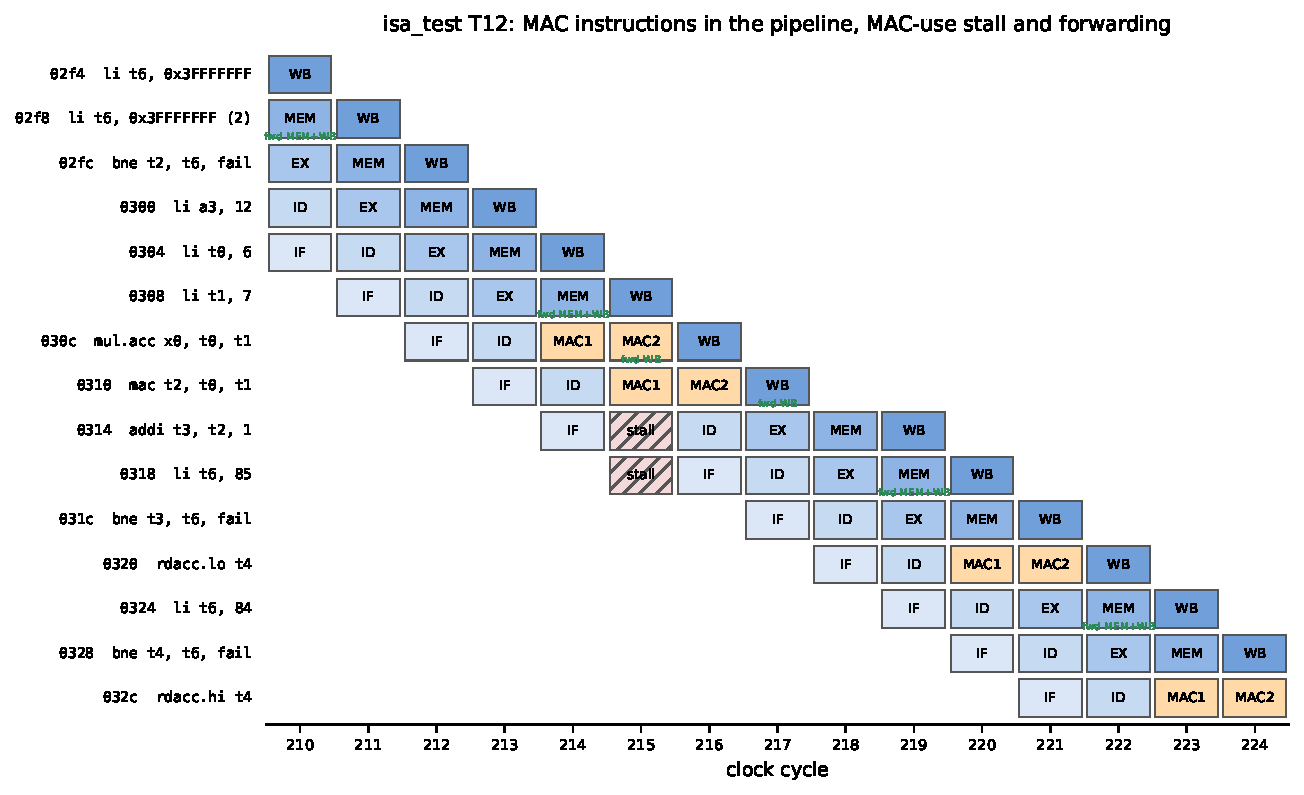
\includegraphics[width=\linewidth]{figures/pipe_isa_mac_hazard.pdf}
  \caption{\code{isa\_test} T12 executing: \code{mul.acc}, \code{mac} and the
    dependent \code{addi t3,t2,1}. The \code{addi} is held in ID for one cycle
    (MAC-use stall) and then receives \code{t2} from WB; the result is 85 as
    expected.}
  \label{fig:pipe_isa}
\end{figure}

In Figure~\ref{fig:pipe_isa}, \code{mul.acc} and \code{mac} occupy MAC1/MAC2
in consecutive cycles without any interference, because the accumulator is
read and written only in MAC stage~2. The instruction that consumes the MAC
result is stalled once by the hazard unit and then gets the value forwarded
from WB. This is exactly the behaviour designed in Chapter~\ref{ch:cpu}.

\begin{figure}[H]
  \centering
  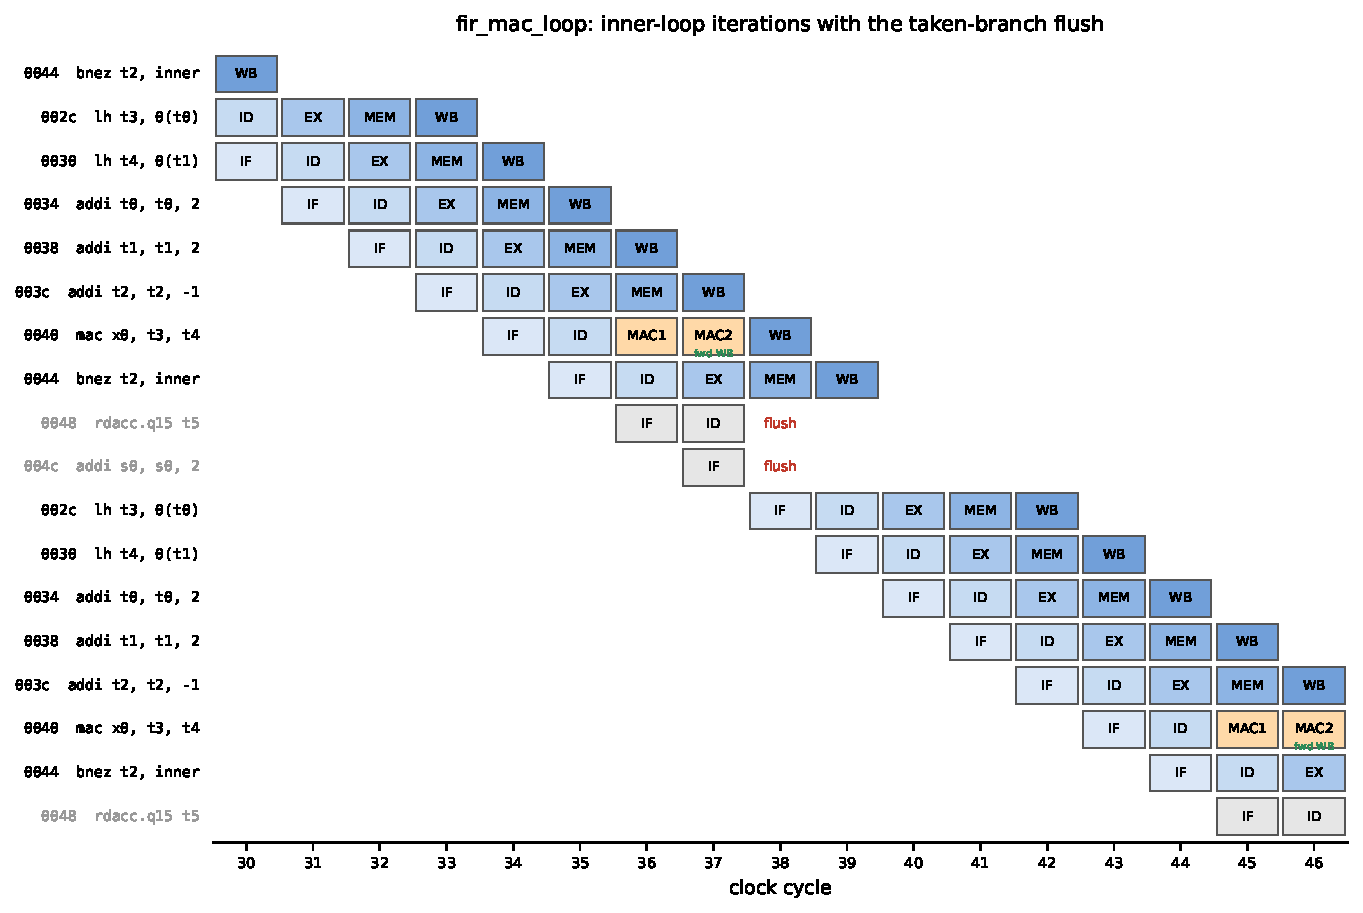
\includegraphics[width=\linewidth]{figures/pipe_fir_loop.pdf}
  \caption{\code{fir\_mac\_loop}: two iterations of the inner loop. Every
    iteration ends with a taken \code{bnez}, which squashes the two
    instructions fetched behind it (2-cycle penalty).}
  \label{fig:pipe_fir}
\end{figure}

\begin{figure}[H]
  \centering
  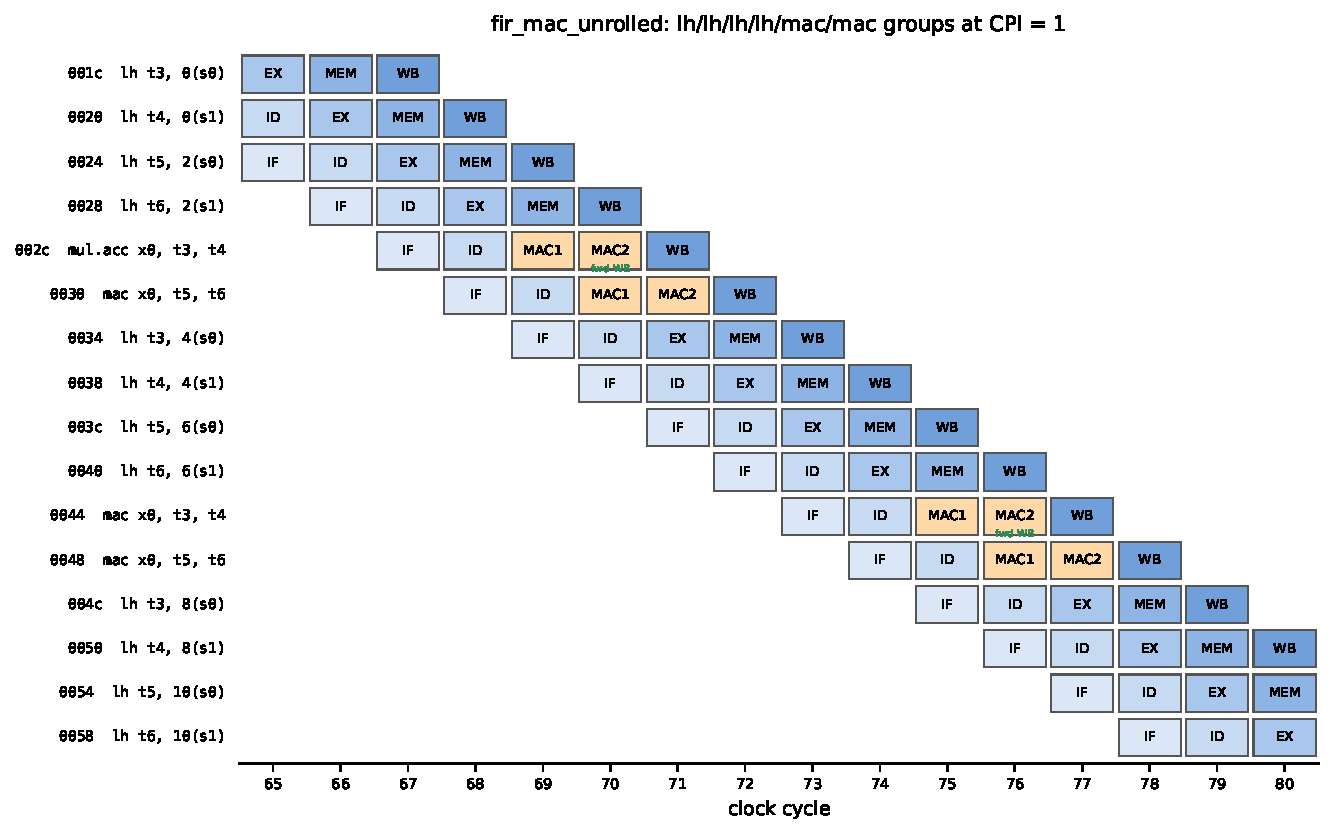
\includegraphics[width=\linewidth]{figures/pipe_fir_unrolled.pdf}
  \caption{\code{fir\_mac\_unrolled}: the unrolled \code{lh}/\code{lh}/\code{lh}/\code{lh}/\code{mac}/\code{mac}
    pattern issues one instruction per cycle with no stalls or flushes.}
  \label{fig:pipe_unrolled}
\end{figure}

Figure~\ref{fig:pipe_fir} explains why the looped FIR has a CPI of 1.26: the
taken branch at the end of each 7-instruction iteration wastes 2 of every
9 cycles. Unrolling (Figure~\ref{fig:pipe_unrolled}) removes the branches
from the tap loop. The pipeline then reaches CPI~1.037, and the MAC unit
receives a new operand pair every third cycle (\code{lh}, \code{lh},
\code{mac}).

\section{Processor waveform}
Figure~\ref{fig:wave_cpu} shows the VCD waveform of \code{fir\_mac\_loop}
around the end of output sample $y[2]$. The first five rows show which
instruction is in each pipeline stage. Note the bubbles after the taken
\code{bnez} and the \code{mac} moving from EX to MEM to WB. The orange rows
show the MAC unit itself. The \code{valid\_i} signal is high while a \code{mac}
is in EX, and its operands $x[n]$ and $h[k]$ (for example $-2708$ and $-114$)
arrive through the forwarding network. One cycle later, the Booth product
appears in \code{s1\_prod} ($-2708\times-114 = 308{,}712$), and one cycle after
that the accumulator updates ($-1{,}731{,}669 + 308{,}712 = -1{,}422{,}957$).
After the loop exits, \code{rdacc.q15} writes
$\lfloor -1{,}422{,}957 / 2^{15}\rfloor = -44$ to register \code{t5} (x30),
and the following \code{sh} stores it as $y[2]$. This value matches the
golden model.

\begin{landscape}
\begin{figure}[p]
  \centering
  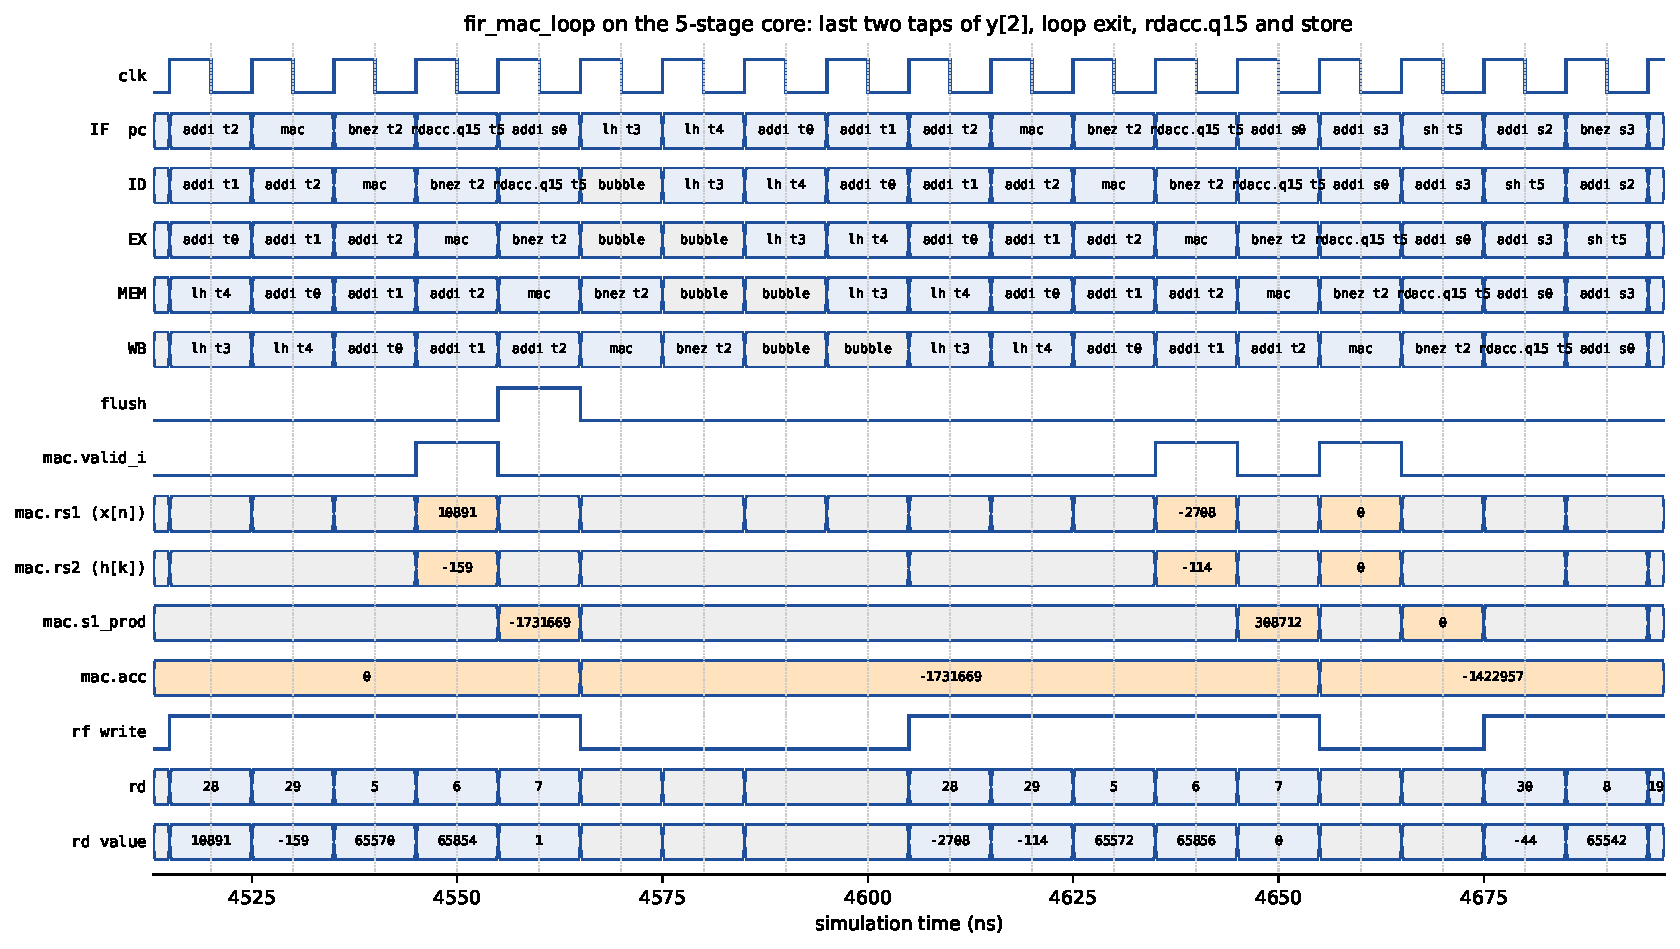
\includegraphics[width=\linewidth]{figures/wave_cpu_mac.pdf}
  \caption[Simulation waveform of the 5-stage core executing the FIR program]{Simulation waveform of the 5-stage core executing \code{fir\_mac\_loop}
    (from \code{sim/cpu/fir\_mac\_loop.vcd}). Pipeline-stage rows show the
    instruction in each stage (grey = bubble); orange rows are MAC-unit
    signals; bus values are blanked while their valid signal is low.}
  \label{fig:wave_cpu}
\end{figure}
\end{landscape}

\section{DSP results: the FIR filter on the processor}
Figure~\ref{fig:fir_time} shows the input signal and the output that the
processor computed with the MAC instructions. The high-frequency tone is
removed and the wanted tone passes through, delayed by the filter's group
delay of 7.5 samples. The lower panel shows two error curves. The difference
from the golden model is \textbf{exactly zero} for all 128 samples, while the
difference from an ideal floating-point filter is at most 2.5\,LSB (1.2\,LSB
rms), which is just the Q15 quantisation of the taps and the signal.

\begin{figure}[H]
  \centering
  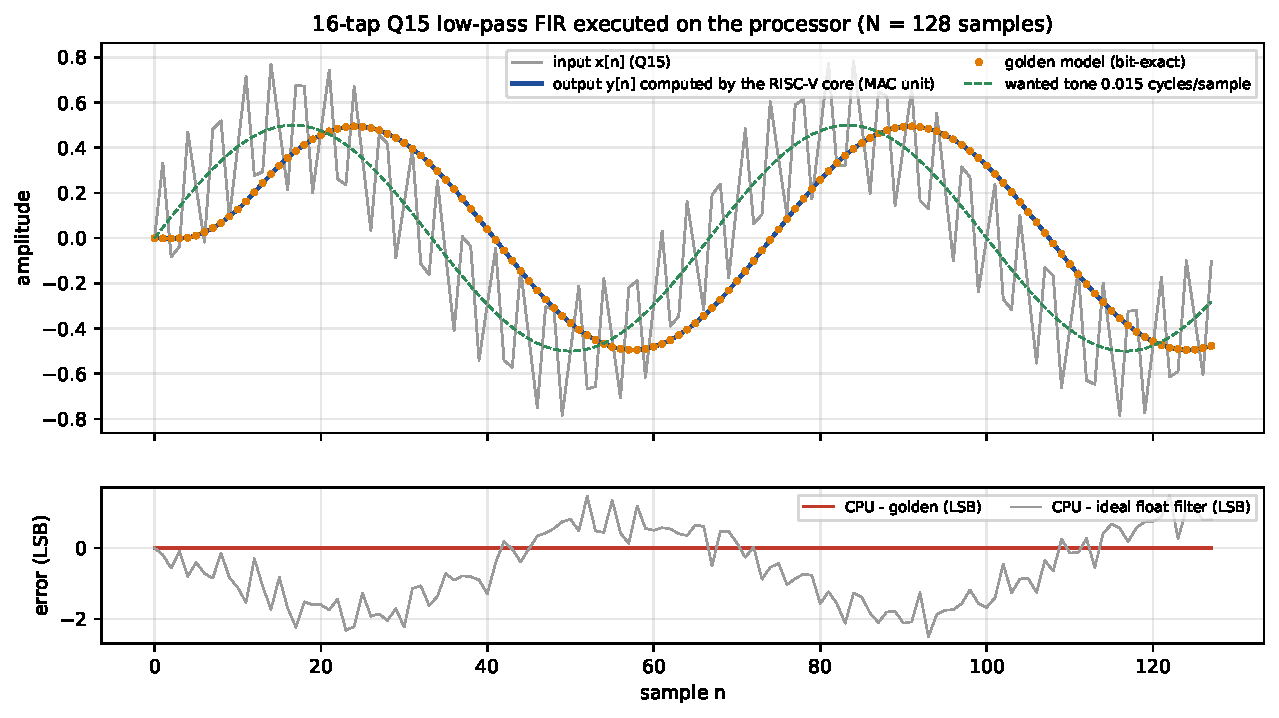
\includegraphics[width=\linewidth]{figures/fir_time.pdf}
  \caption{FIR filtering executed on the RISC-V core: input, CPU output and
    golden model (top), and the error against the golden model and against
    an ideal floating-point filter (bottom).}
  \label{fig:fir_time}
\end{figure}

The spectra in Figure~\ref{fig:fir_spec} quantify the result. The unwanted
tone at 0.3 cycles/sample drops from $-11.3$\,dBFS to $-71.4$\,dBFS, an
attenuation of \textbf{60.1\,dB}, which agrees with the filter's theoretical
response $|H(0.3)| = -60.2$\,dB (Figure~\ref{fig:fir_h}). The wanted tone at
0.015 cycles/sample, by contrast, changes by only $-0.1$\,dB.

\begin{figure}[H]
  \centering
  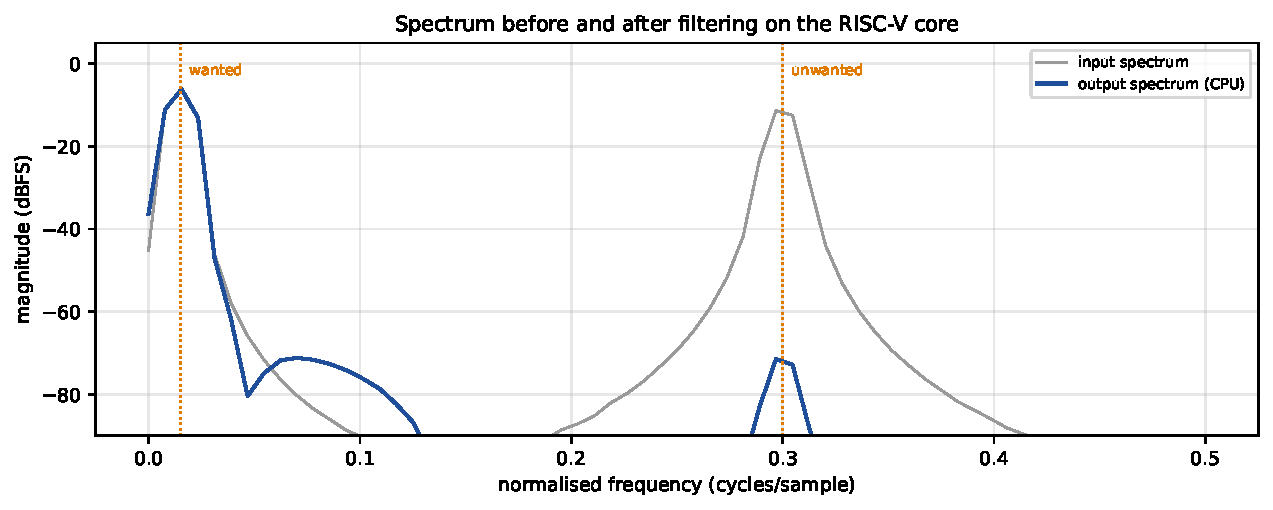
\includegraphics[width=\linewidth]{figures/fir_spectrum.pdf}
  \caption{Spectrum of the input and of the output computed by the processor.}
  \label{fig:fir_spec}
\end{figure}

\begin{figure}[H]
  \centering
  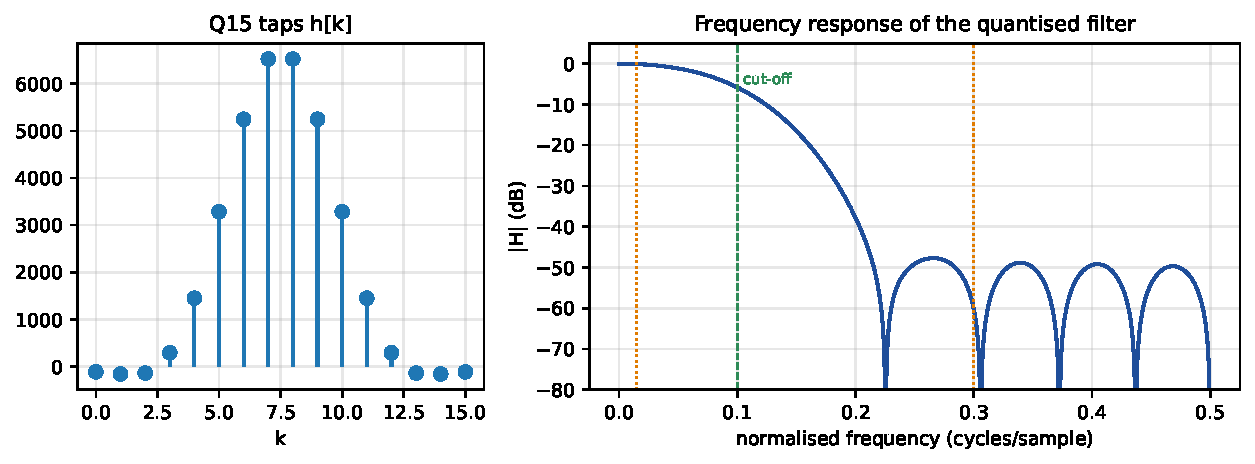
\includegraphics[width=\linewidth]{figures/fir_freqresp.pdf}
  \caption{Quantised Q15 filter taps and frequency response.}
  \label{fig:fir_h}
\end{figure}

\section{Performance: MAC unit vs.\ plain RV32IM}
Because both versions of the filter run on the same core and produce the same
bit-exact output, their cycle counts can be compared directly
(Figure~\ref{fig:perf}, Table~\ref{tab:speedup}).

\begin{figure}[H]
  \centering
  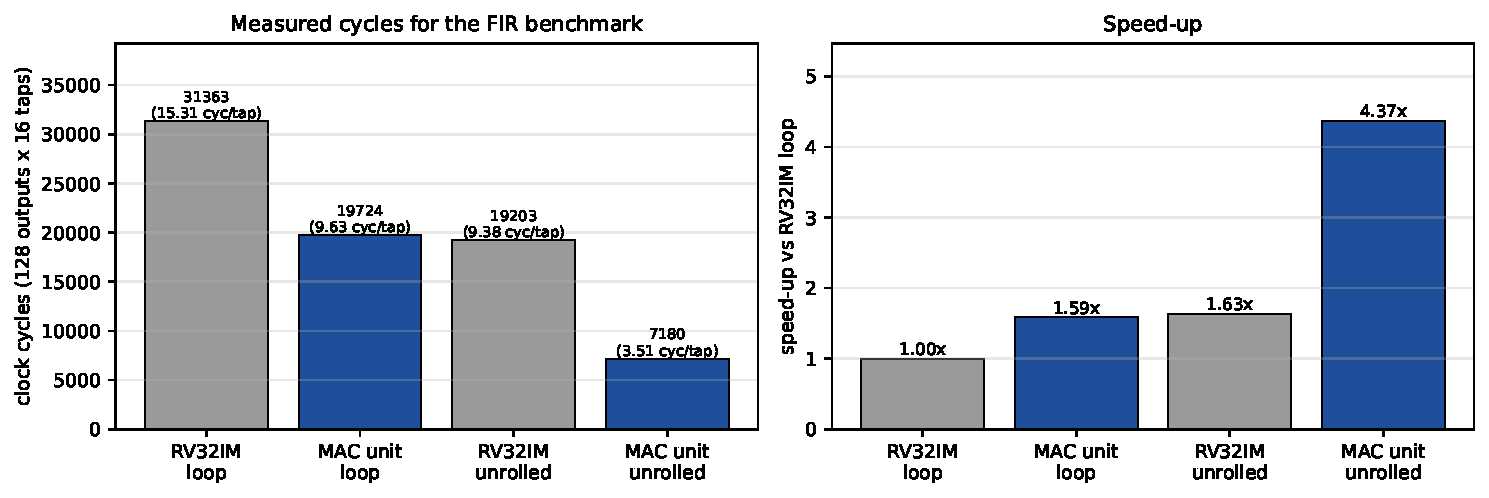
\includegraphics[width=\linewidth]{figures/perf_cycles.pdf}
  \caption{Measured FIR execution time (128 outputs $\times$ 16 taps) and speed-up.}
  \label{fig:perf}
\end{figure}

\begin{table}[H]
  \centering
  \caption{FIR benchmark: MAC instructions vs.\ RV32IM software (measured).}
  \label{tab:speedup}
  \small
  \begin{tabular}{@{}lrrrrr@{}}
    \toprule
    Version & Cycles & Cycles/tap & Instructions & Code size & Speed-up \\
    \midrule
    RV32IM loop             & 31{,}363 & 15.31 & 26{,}895 &  51 instr. & 1.00$\times$ \\
    MAC loop                & 19{,}724 &  9.63 & 15{,}626 &  27 instr. & \textbf{1.59$\times$} \\
    RV32IM unrolled         & 19{,}203 &  9.38 & 18{,}575 & 166 instr. & 1.63$\times$ \\
    MAC unrolled            &  7{,}180 &  3.51 &  6{,}922 &  64 instr. & \textbf{4.37$\times$} \\
    \midrule
    MAC vs.\ RV32IM, same code style & \multicolumn{5}{l}{loop: \textbf{1.59$\times$} faster;\quad unrolled: \textbf{2.67$\times$} faster, 2.6$\times$ smaller code} \\
    \bottomrule
  \end{tabular}
\end{table}

Figure~\ref{fig:breakdown} shows where the cycles go, measured with the
performance counters. With the unrolled MAC code, 96\,\% of all cycles retire
a useful instruction, whereas in the looped versions 14--21\,\% of the cycles
are lost to branch flushes. The scheduled FIR code, on the other hand, has no
load-use or MAC-use stalls at all.
At the processor's post-route clock frequency of 34.6\,MHz on the ECP5 FPGA
(Chapter~\ref{ch:synth}), the unrolled MAC version filters one output sample
in 56~cycles (1.6\,$\mu$s, about 616{,}000 samples/s). The unrolled RV32IM
version needs 150~cycles (4.3\,$\mu$s).

\begin{figure}[H]
  \centering
  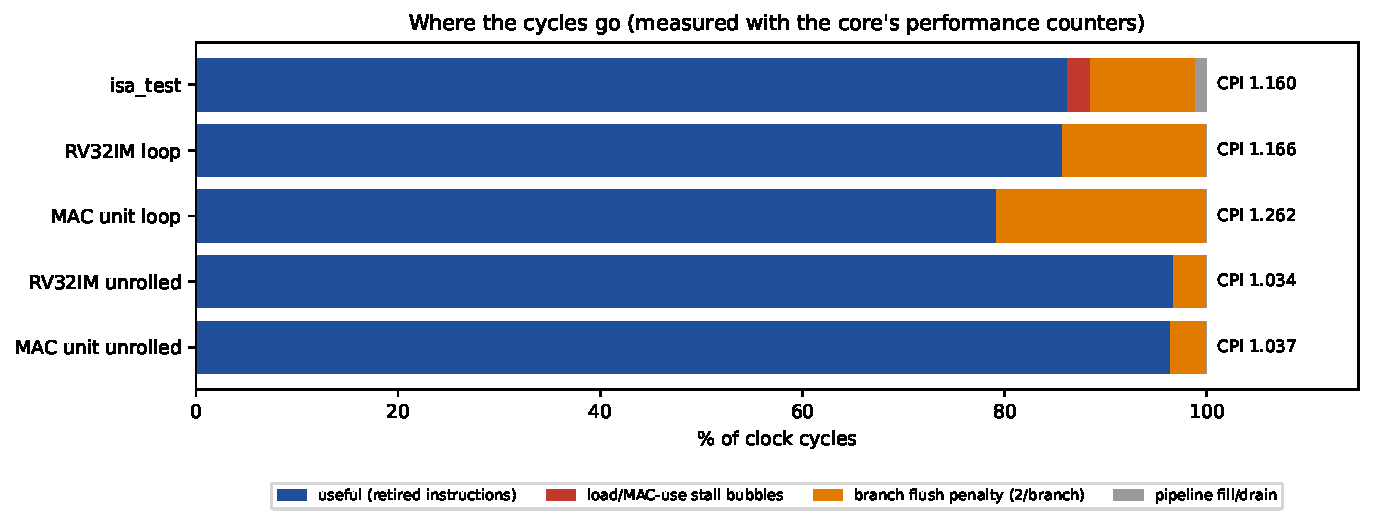
\includegraphics[width=\linewidth]{figures/perf_breakdown.pdf}
  \caption{Cycle breakdown and CPI of every program.}
  \label{fig:breakdown}
\end{figure}
